\documentclass[10pt,conference,compsocconf]{IEEEtran}

%\usepackage{times}
%\usepackage{balance}
\usepackage{url}
\usepackage{graphicx}	% For figure environment

\usepackage{booktabs} % For formal tables
\usepackage{xcolor}

\usepackage{multirow}

% Make TODOs an error by out commenting the command.
%\newcommand{\TODO}[1]{\{\textbf{TODO: }\textcolor{red}{#1}\}}
\usepackage{pdfpages}

\IEEEoverridecommandlockouts %Enables \thanks to be used again

\begin{document}
\title{Computational Intelligence Lab: Tweet Sentiment Classification}

\author{
  Luk\'{a}\v{s} Jendele$^\ast$\\
  ETH Z\"{u}rich\\
  \texttt{jendelel@ethz.ch}\\
  \and
  Larissa Laich$^\ast$\\
  ETH Z\"{u}rich\\
  \texttt{llaich@ethz.ch}\\
  \and
  Ondrej Skopek$^\ast$\\
  ETH Z\"{u}rich\\
  \texttt{oskopek@ethz.ch}\\
  \and
  Michael Wiegner$^\ast$\thanks{$^\ast$ All authors contributed equally.}\\
  ETH Z\"{u}rich\\
  \texttt{wiegnerm@ethz.ch}\\
}

\maketitle%

\begin{abstract}
Sentiment analysis is a key stepping stone on the path to natural language understanding. In this paper, we show that deep neural networks can learn to classify sentiment even on very short and noisy texts with almost no preprocessing, by evaluating our models on the Twitter dataset and obtaining competitive results (88.5\% test set accuracy). We investigated the performance of different Recurrent and Convolutional Neural Network based models on the binary sentiment classification problem and compared all our approaches to simpler baselines.
\end{abstract}

\section{Introduction}
With the rise of Internet technologies, micro-blogging sites like Twitter have became increasingly popular to share and discuss information and express personal opinions. Used by millions of people on a daily basis, Twitter has become a source of data and offers huge opportunities for analysis. One of many applications is for example market analysis: how users perceive certain companies' products. Due to the large amount of data, reliable automated sentiment analysis is essential to be able to process and extract information from it efficiently. Recent developments in machine learning, like deep neural networks have shown promising results when performing sentiment analysis. However, there is still room for improvement, which is what we want to investigate in this paper. In our task, we classify tweets based on positive or negative sentiment.

Tweets are short messages on Twitter which were originally limited to a length of 140 characters. Due to this length limitation and the fact that it is a fast-paced micro-blogging platform, most people use abbreviations, emoticons, hashtags, or ``@username'' to refer to other users. The dataset is therefore relatively structured and allows us to determine sentiment by checking emoticons occurring in tweets. Tweets with a ``:)'' smiley are considered to be positive tweets while negative tweets contain a ``:('' smiley. This allows us to label the data automatically as the smilies are removed from the training data and used as a label. Determining tweet sentiment simply based on an emoticon contained in the tweet introduces some noise to the labels, as there sometimes is not a direct correlation between sentiment and smiley (e.g.~irony, sarcasm, \ldots). On the other hand, the use of colloquial language makes this task different from analyzing text from books or articles, and reflects the rough real world conditions of language use. 

For this project, we designed and implemented multiple machine learning models for sentiment analysis. The results are evaluated based on classification accuracy.
Our contributions are the following:
\begin{enumerate}
\item Improved accuracy from the best baseline models by approximately 7\%.
\item By using ensembles, improved performance by another 0.5\%.
\item Achieved 3\textsuperscript{rd} best result on both public and private Kaggle test datasets.
\end{enumerate}

\section{Related work}
Sentiment analysis is one the most basic text classification tasks, and therefore, has been a subject of interest to many researchers
\cite{TextCNN,mozetivc2016multilingual,transformer,twitter_preprocessing,CharTextCNN}. 
While part of the research focused on data preprocessing \cite{twitter_preprocessing}, others were more concerned with the classification model itself \cite{TextCNN}.

Before deep learning models, researchers extracted features from the text and ran a binary classifier on these features \cite{features}, as recommended in the CIL course tutorial.

With the recent success of deep neural networks in natural language processing problems, researchers tackled sentiment analysis by applying various convolutional \cite{TextCNN} and recurrent neural networks \cite{rnn} to the task. 

In our approach, we implemented both classical, as well as modern neural network approaches, apply them to sentiment analysis and compare them with each other.

\section{Models and Methods}

We use several different approaches to classify sentiment. In this section, we briefly describe each model and explain our motivation for its usage.

\begin{figure}
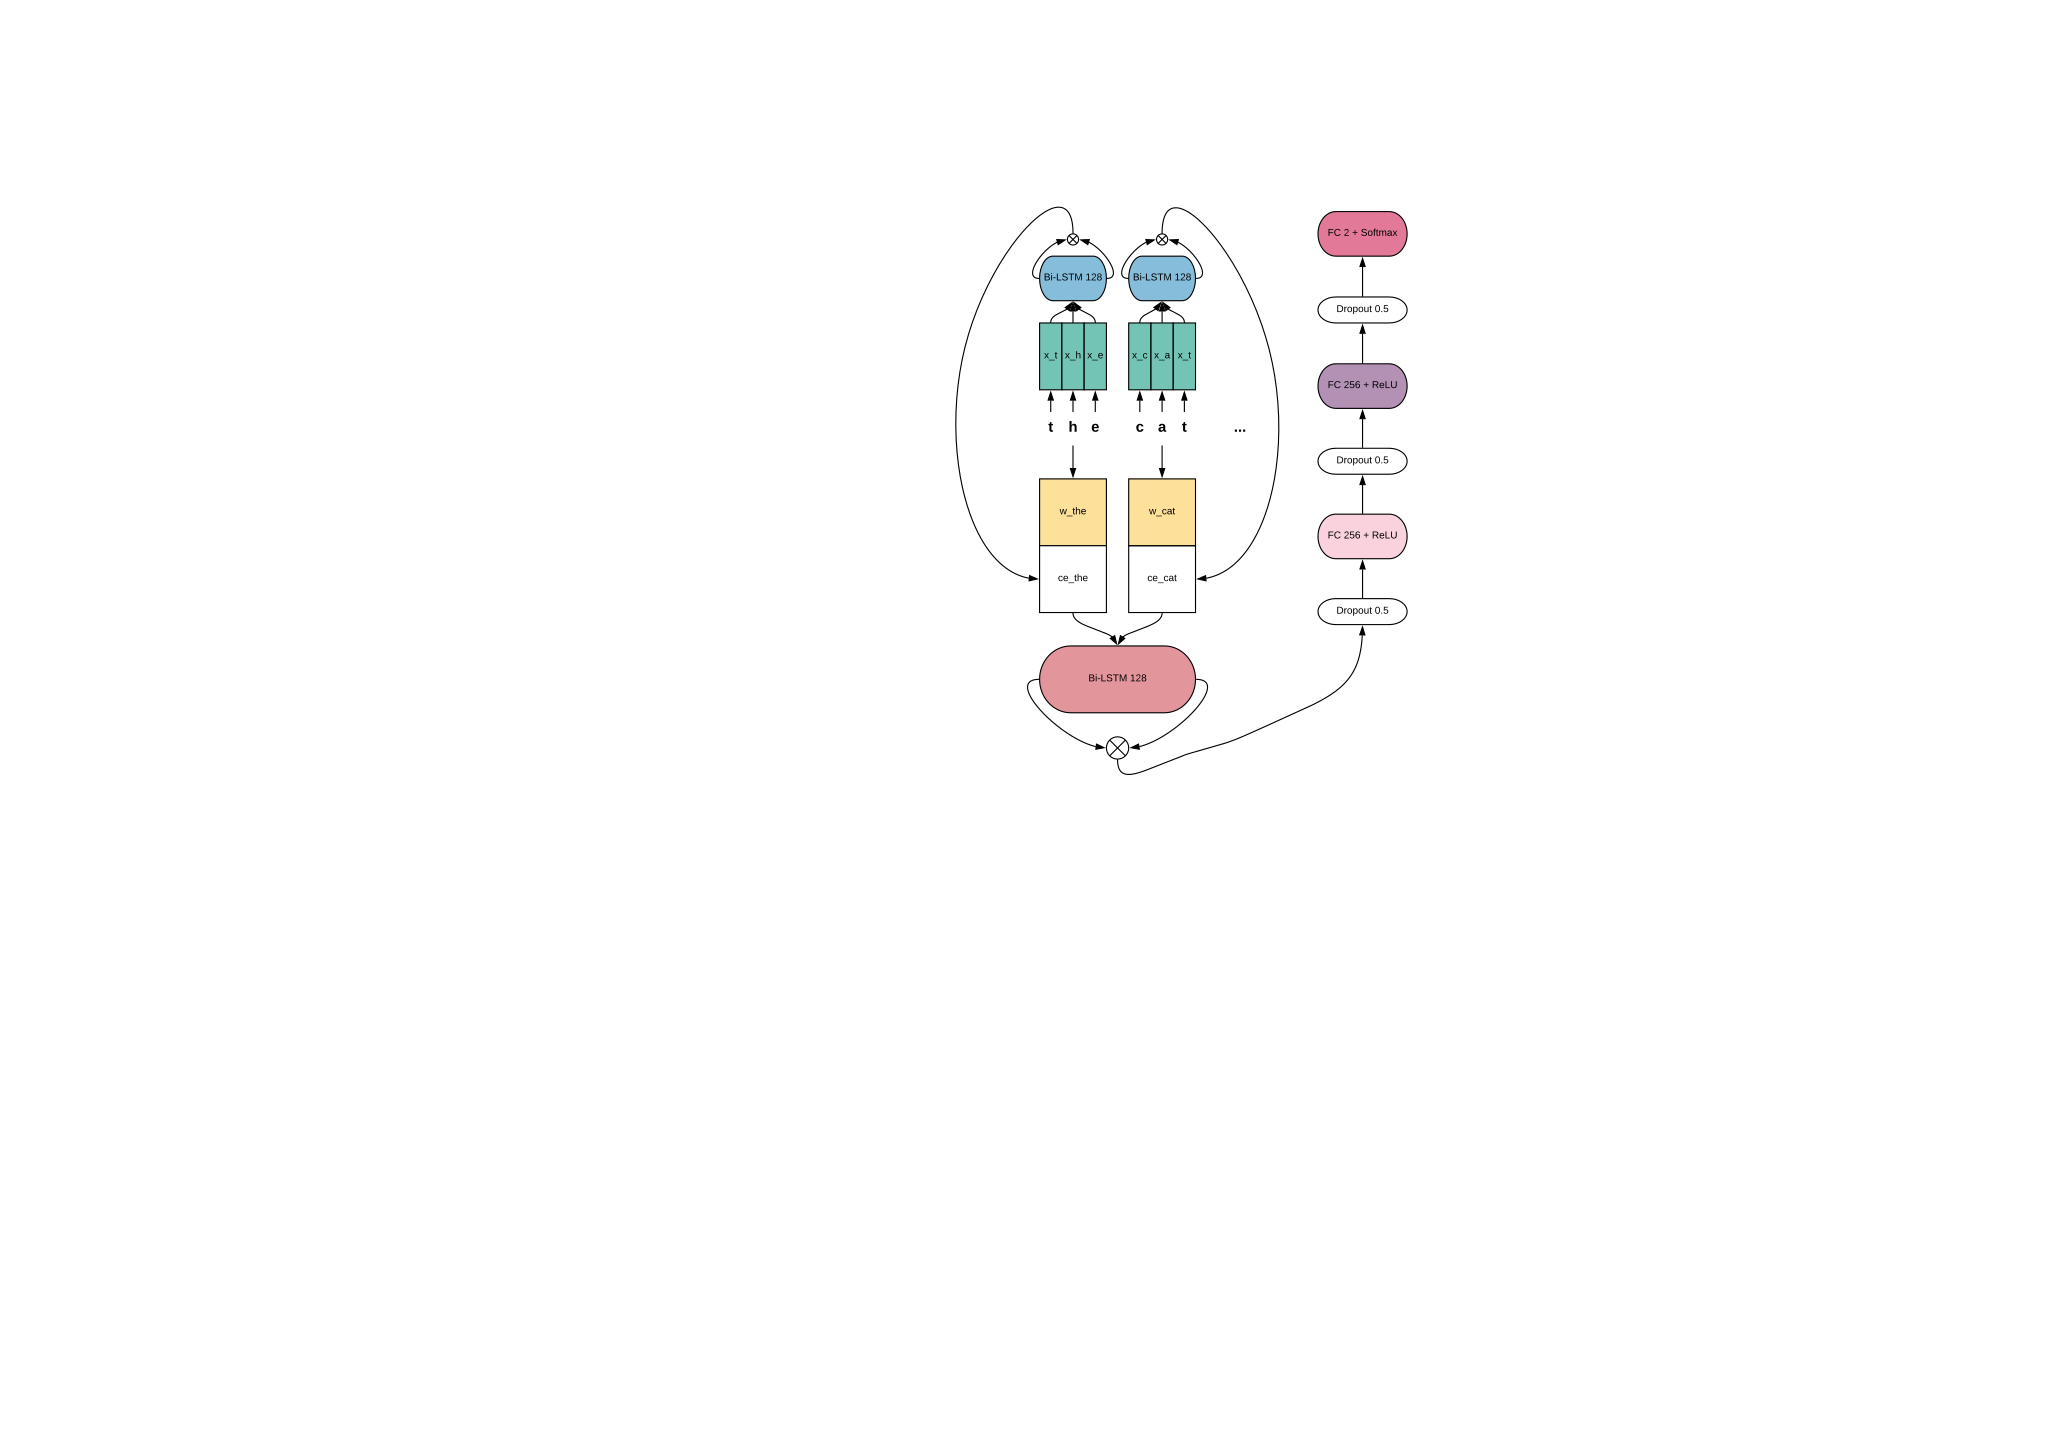
\includegraphics[width=0.48\textwidth]{./rnn}
\caption{Sketch of our recurrent neural network architecture LSTM128. Equal colors indicate shared weights. $x\_$ represent individual character embeddings, $w\_$ represent word embeddings, and $ce\_$ represent character-based word embeddings.
The $\otimes$ symbol indicates concatenation.}
\label{fig:arch}
\end{figure}

\subsection{Baselines}
%In order to compare our models, we implemented three baselines.

\subsubsection{Glove + Logistic regression}
This baseline is taken from the CIL lecture. We use GloVe word embeddings \cite{pennington2014glove} and average them for each tweet. On the resulting vector, we apply logistic regression. For this baseline, we either compute the Glove embeddings based on our training data by using scripts from the CIL tutorial, or use precomputed ones from Stanford University\footnote{\url{https://nlp.stanford.edu/projects/glove/}}.
Both variants of the embeddings have 200 dimensions.

\subsubsection{Glove + Random Forest}
Similarly to the previous baseline, we average the GloVe word embeddings for each tweet. However, this time we use a Random Forest (RF) classifier \cite{random-forests} with 128 trees. We report scores for evaluation using both the self trained and Stanford pre-trained Glove embeddings. The same dimensionality as above was used.

\subsubsection{FastText}
FastText \cite{joulin2017bag} is a command-line tool developed by Facebook AI Research. As it is simple to set up and runs fast, we decided to run it on our dataset and consider it as one of the baselines. In one step, it learns word embeddings in an unsupervised way, and trains a simple classifier on them. 

\subsection{Common preprocessing}
For our RNN and CNN models, we apply a common loading and preprocessing step. As the input data is already lowercased and spaces are normalized, we only apply a vocabulary downsize and padding step for computational reasons.
We only add the 20 000 most common words (in the training data) to our vocabulary. All other words are mapped to an UNK token. Moreover, we clip tweets at 40 words (only very few tweets are longer than that).

We also experimented with more heavy preprocessing similar to \cite{twitter_preprocessing}, but did not manage to achieve significant improvements in performance compared to the un-preprocessed variant of our models.

\subsection{RNN models}
Recurrent neural networks are one of the most used network architectures for natural language processing tasks such as machine translation, language modeling, and text classification.

Our model architecture is depicted in Figure~\ref{fig:arch}. First, we run a bi-directional RNN on each of the tweet words' embedded characters. We concatenate the final hidden states with randomly initialized whole-word embeddings, and use the concatenated vectors as the final word embeddings for the next layer.
Another bi-directional RNN network is run on the final word embeddings and its hidden states are fed into two 256-unit fully connected layers with ReLU activation functions and dropout \cite{dropout1,dropout2} in between them (with keep probability 0.5). Finally, we append a fully connected layer with Softmax that classifies into positive and negative labels,
and train the network using a cross-entropy loss function. 

We use only two RNN cells with dimensionality of the hidden state(s) 128, one for the character RNN and one for the word RNN. A single cell is used for both directions. Our character and word embeddings have 200 dimensions. 

We also briefly experimented with both Luong \cite{luong} and Bahdanau \cite{bahdanau} attention, but only observed higher training times and equivalent performance to models without attention.

The performance of the model depends largely on the recurrent cell. Thus, we ran the described architecture with minor changes (each described below) and report the performance.

\subsubsection{LSTM128}
Long-Short-Term-Memory \cite{lstm} cells are the most frequently used recurrent units used to process text. They are well-known for their ability to capture long-range contextual features in text. In our implementation, the cell's hidden state has 128 dimensions, and we concatenate both final cell state and final hidden state of the cell. Then we concatenate the forward and backward states of the bi-directional RNN and pass the result to the fully-connected layers.

\subsubsection{GRU256}
Gated Recurrent Unit \cite{gru} has proven to be the best compromise of learning capabilities and computational complexity. It contains less gating (only one hidden state) than the more popular and older LSTM cell. Therefore, we ran an experiment in which we replaced the LSTM cell with a GRU cell of dimensionality 256.

\subsubsection{LSTM128 without character embeddings}
In this experiment, we removed the first RNN network. That way, we completely ignore word morphology, but acquire a significantly simpler model.

\subsubsection{LSTM128 without word embeddings}
Conversely, we only use the character based part computed by the first RNN here. This enforces a more hierarchical and end-to-end learned model.

\subsubsection{Stacked LSTM}
To increase the model's capacity (its power to learn), we stack multiple LSTM cells on top of each other, which is a common practice in machine translation models \cite{zeroshot}. For our purposes, we use two LSTMs, with dropout with a keep probability of 0.5 on all individual LSTM cell inputs and outputs.


\subsection{Other models}

\subsubsection{TextCNN}
Recurrent neural networks are well known for their capabilities to capture long context. However, tweets are very short and therefore a limited fixed receptive field is most likely capable of learning the text sentiment. Thus, we replaced the word RNN with convolutions similar to \cite{TextCNN}. We used kernel sizes 3, 4, 5, and 7, each with 512 channels (model implementation is called CNN512).

\subsubsection{Transformer Tiny}
Transformer \cite{transformer} is a state of the art method in machine translation. It uses gating similar to RNN cells, while processing tokens in parallel similar to CNNs. We utilized the Tensor2Tensor \cite{tensor2tensor} implementation, and trained the ``tiny'' version (2 hidden layers) of the model's encoder for classification.

\subsubsection{Ensemble Majority Vote}
Motivated by most data science competitions, an ensemble of several strong models usually yields to better performance. Thus, to lower the prediction variance, we combined the test predictions of several different approaches using majority voting: LSTM128, Stanford GloVe+RF, Transformer, Stacked LSTM, and CNN. We decided to select five models as an odd number always leads to a majority vote for one of the two labels. Additionally, a single model still has some weight when we choose a relatively small number of models.

\subsection{Implementation}
All neural network models are implemented in TensorFlow \cite{tensorflow}, and trained with the Adam optimizer \cite{adam} with a learning rate of $3 \cdot 10^{-4}$. All variables were initialized with Glorot initialization \cite{glorot2010understanding}.
The GloVe embedding implementation was adapted from the coding exercise solution to CIL tutorial 6. When training GloVe embeddings, we train for 20 epochs. For the Random Forests and Logistic Regression, we used the NumPy \cite{numpy} and scikit-learn \cite{scikit-learn} Python libraries.
For FastText and Transformer, we used the original implementations available online\footnote{\url{https://fasttext.cc/}, \url{https://github.com/tensorflow/tensor2tensor}}.
The ensemble majority voting was done in a simple spreadsheet.

All code is available in the repository\footnote{\url{https://github.com/oskopek/cil}} and is also attached to our paper submission.


\section{Experiments}
To achieve reproducible results, we trained all experiments with the same fixed random seed. Moreover, we split the data into a training and evaluation set which we used for all the experiments.
The evaluation set contained 100 000 tweets, and the remaining 2.4 million tweets were used for training.

All neural network experiments were trained on the Leonhard ETHZ cluster on a single Nvidia GeForce GTX 1080 Ti GPU.
All of our experiments ran for a maximum of 24 hours, 15 epochs,
with batch size 32.
We evaluated on the full evaluation set every 7500 steps (independent on the batch size), and as the final predictions, used the ones that were created at the point where the model had the highest evaluation accuracy.
Most models obtained best results around epochs 9--12, which corresponds
to about 21 hours in training time.
The Stacked LSTM ran with batch size 256 for about 12 hours.

The Transformer was trained for 40 000 steps in mini-batches of 8 000 words. The model trains for about an hour, which is significantly faster than all of the RNN based models.

FastText ran for a very short time on commodity CPU hardware.
Due to its instability, with respect to the random seed,
we perform 5 runs, and report the standard deviations. 

Our GloVe implementation consumes a lot of memory (peak at $\approx$ 40 GB), and runs for about 2-3 hours on a CPU.
  
\section{Results}

\begin{table}\centering
\begin{tabular}{lrrr}
\toprule
\multirow{2}{*}{Model} & \multicolumn{1}{c}{Evaluation} & \multicolumn{1}{c}{Test (public)} & \multicolumn{1}{c}{Test (private)}\\
& Acc.~\% & Acc.~\% & Acc.~\%\\
\midrule
GloVe + LR & 61.69 & 61.56 & 62.10\\
Stanford GloVe + LR & 78.08 & 77.06 & 76.94\\
GloVe + RF & 71.00 & 67.84 & 69.04\\
Stanford GloVe + RF & 79.97 & 77.00 & 77.94\\
FastText \cite{joulin2017bag} & \textbf{81.31} \textbf{$\pm$ 2.21} & \textbf{80.88 $\pm$ 2.03}& \textbf{80.50 $\pm$ 1.57}\\
\midrule
knilpt &  & \textbf{89.08} & 88.48\\
Satisfaction &  & 88.78 & \textbf{88.62}\\
\midrule
LSTM128 & 88.49 & 87.90 & 87.82\\
GRU256 & 88.45 & 87.66 & 87.52\\
LSTM128 w/o WE & 87.88 & 86.98 & 86.56\\
LSTM128 w/o CE & 88.18 & 87.82 & \textbf{87.90}\\
Stacked LSTM & \textbf{88.58} & 88.06 & 87.68\\
TextCNN & 87.71 & 87.70 & 87.10\\
Transformer Tiny & 86.00 & 85.34 & 83.84\\
Ensemble Majority Vote & & \textbf{88.54} & 87.78\\
\bottomrule
\end{tabular}
\caption{Evaluation and test set results. Values left blank are unknown. Acc.~means accuracy, LR~is logistic regression, WE/CE are word/character embeddings respectively, and RF denotes a Random Forest. The top section describes baselines that we ran on our data split. Middle section contains the two top teams on Kaggle for this project. Bottom section shows our results. Values that have confidence intervals were unstable enough to be have to be run 5 times.}\label{tab:results}
\end{table}

The results of all our experiments are summarized in Table~\ref{tab:results}. The reported evaluation accuracy is the best one obtained during training (and hence the version of the model with which we submitted the predictions to Kaggle). The public and private test scores correspond to the scores those submissions obtained on the Kaggle data splits. The values left blank are unknown.

In Table~\ref{tab:params}, we present the number of parameters for our models (including the learned embeddings).

\begin{table}\centering
\begin{tabular}{lr}
\toprule
Model & Parameters\\
\midrule
LSTM128 & 4.8 M\\
GRU256 & 5.3 M\\
LSTM128 w/o WE & 0.7 M\\
LSTM128 w/o CE & 4.4 M\\
Stacked LSTM & 21.1 M\\
TextCNN & 11.7 M\\
Transformer Tiny & 1.5 M\\
Ensemble Majority Vote & $\approx$ 51.1 M\\
\bottomrule
\end{tabular}
\caption{Number of parameters of our models.}\label{tab:params}
\end{table}

\section{Discussion}

We can observe that all our models perform consistently better than all baselines, and most also perform better than the best submissions of all teams below us on the Kaggle leaderboard.

An interesting observation is that some models generalize to the test set better than others. For example, the accuracy of TextCNN only drops marginally on the test sets compared to the evaluation set, as opposed to all our RNN models. Generally, we observe that the simpler the model, the better it generalizes (among neural models, e.g.~LSTM128 w/o WE, LSTM128 w/o CE).

As can be seen in Table~\ref{tab:params},
the number of parameters in a model has limited effect on its performance. We can see that above a model complexity, adding more parameters increases the performance; however only marginally. Based on the complexity of the model LSTM model comes out clearly as the best. Despite weaker performance, Transformer's scores are impressive considering the duration of training ($\approx 20\times$\,faster) and lower parameter count. Given enough parameter tweaking, the model has big potential.

\begin{table}\centering
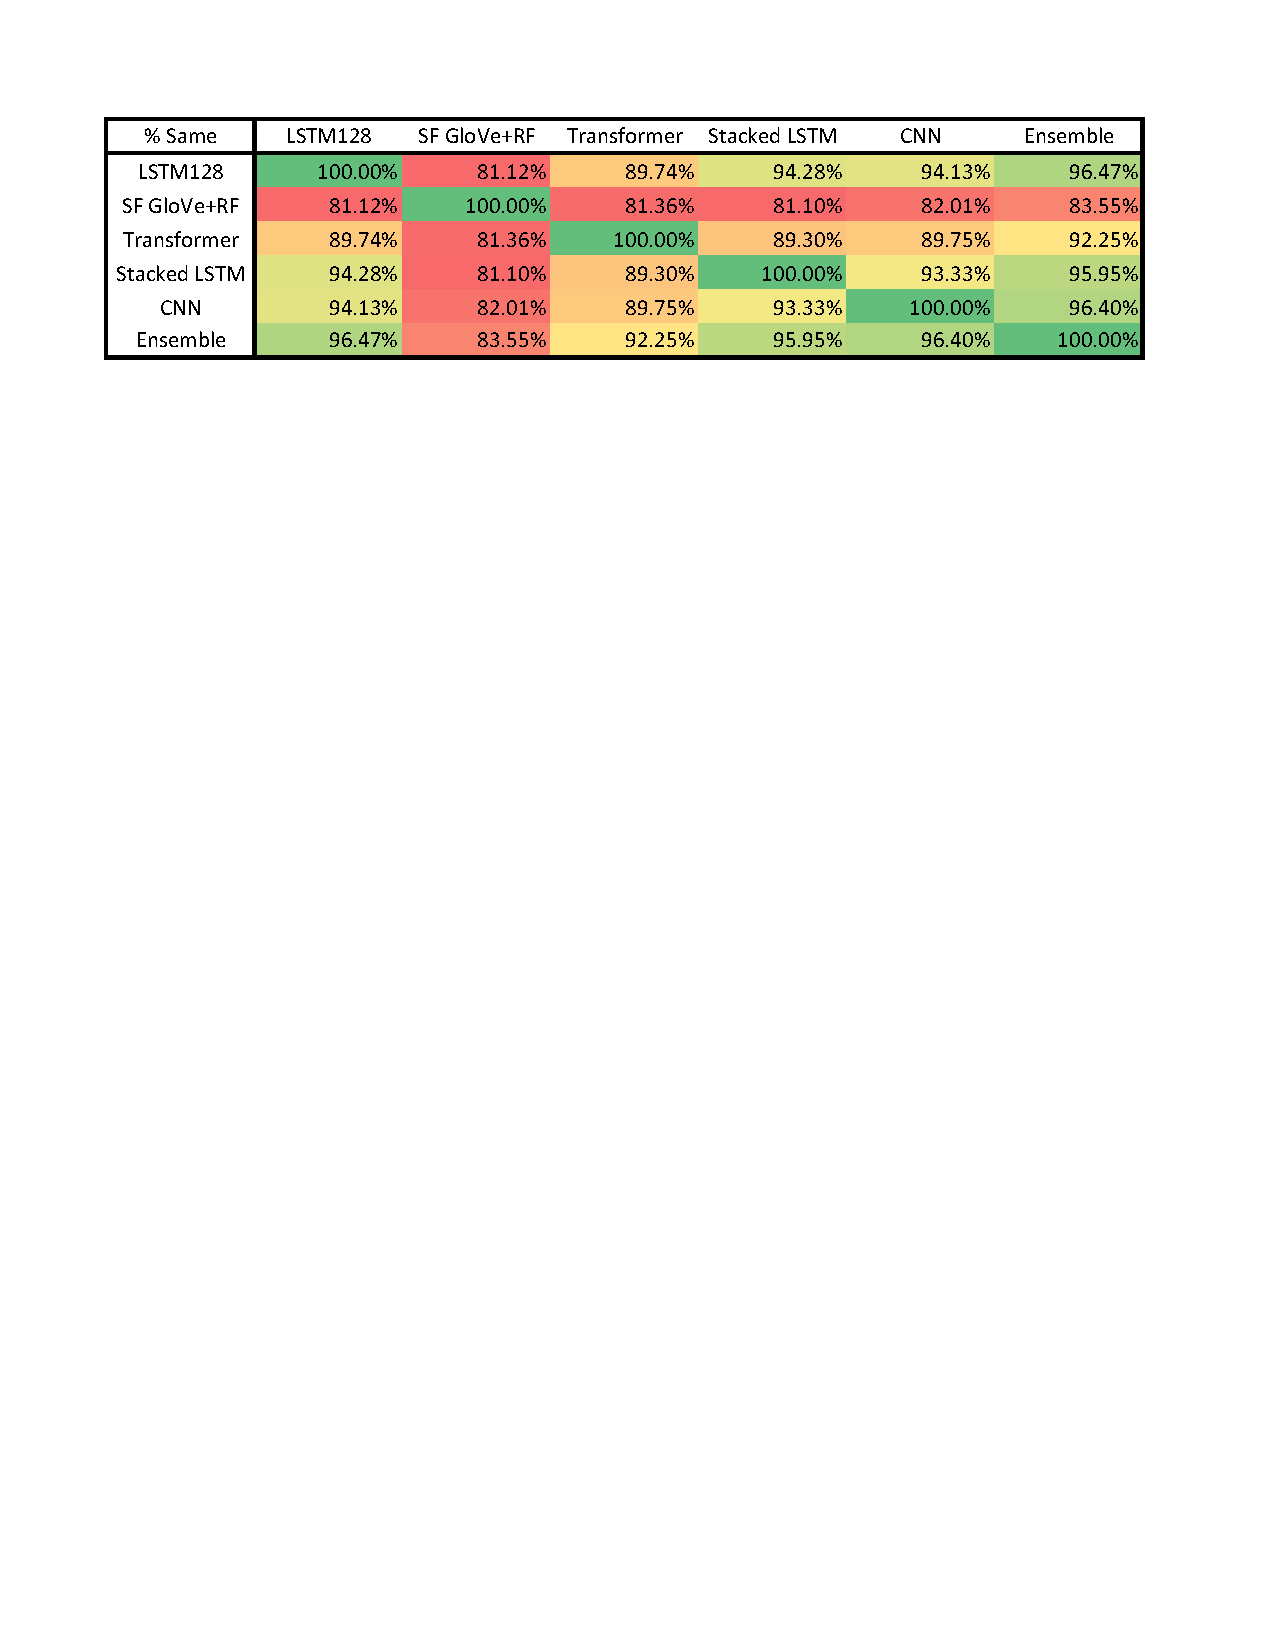
\includegraphics[width=0.48\textwidth]{./ensemble_tablev2}
\caption{Pairwise label agreement between the various models used in the ensemble on the test set. Note that the table is symmetric.}\label{tab:agreement}
\end{table}



An interesting comparison of how surprisingly diverse the models we trained are 
can be seen in Table~\ref{tab:agreement}. Interestingly, our well  performing models (LSTM128, TextCNN, and Stacked LSTM) only agree with each other in about 94\% of the cases (pairwise).
We can also see the effects of lower performance of the Transformer and GloVe+RF models on the pairwise agreement with other models. 

\begin{figure}\centering
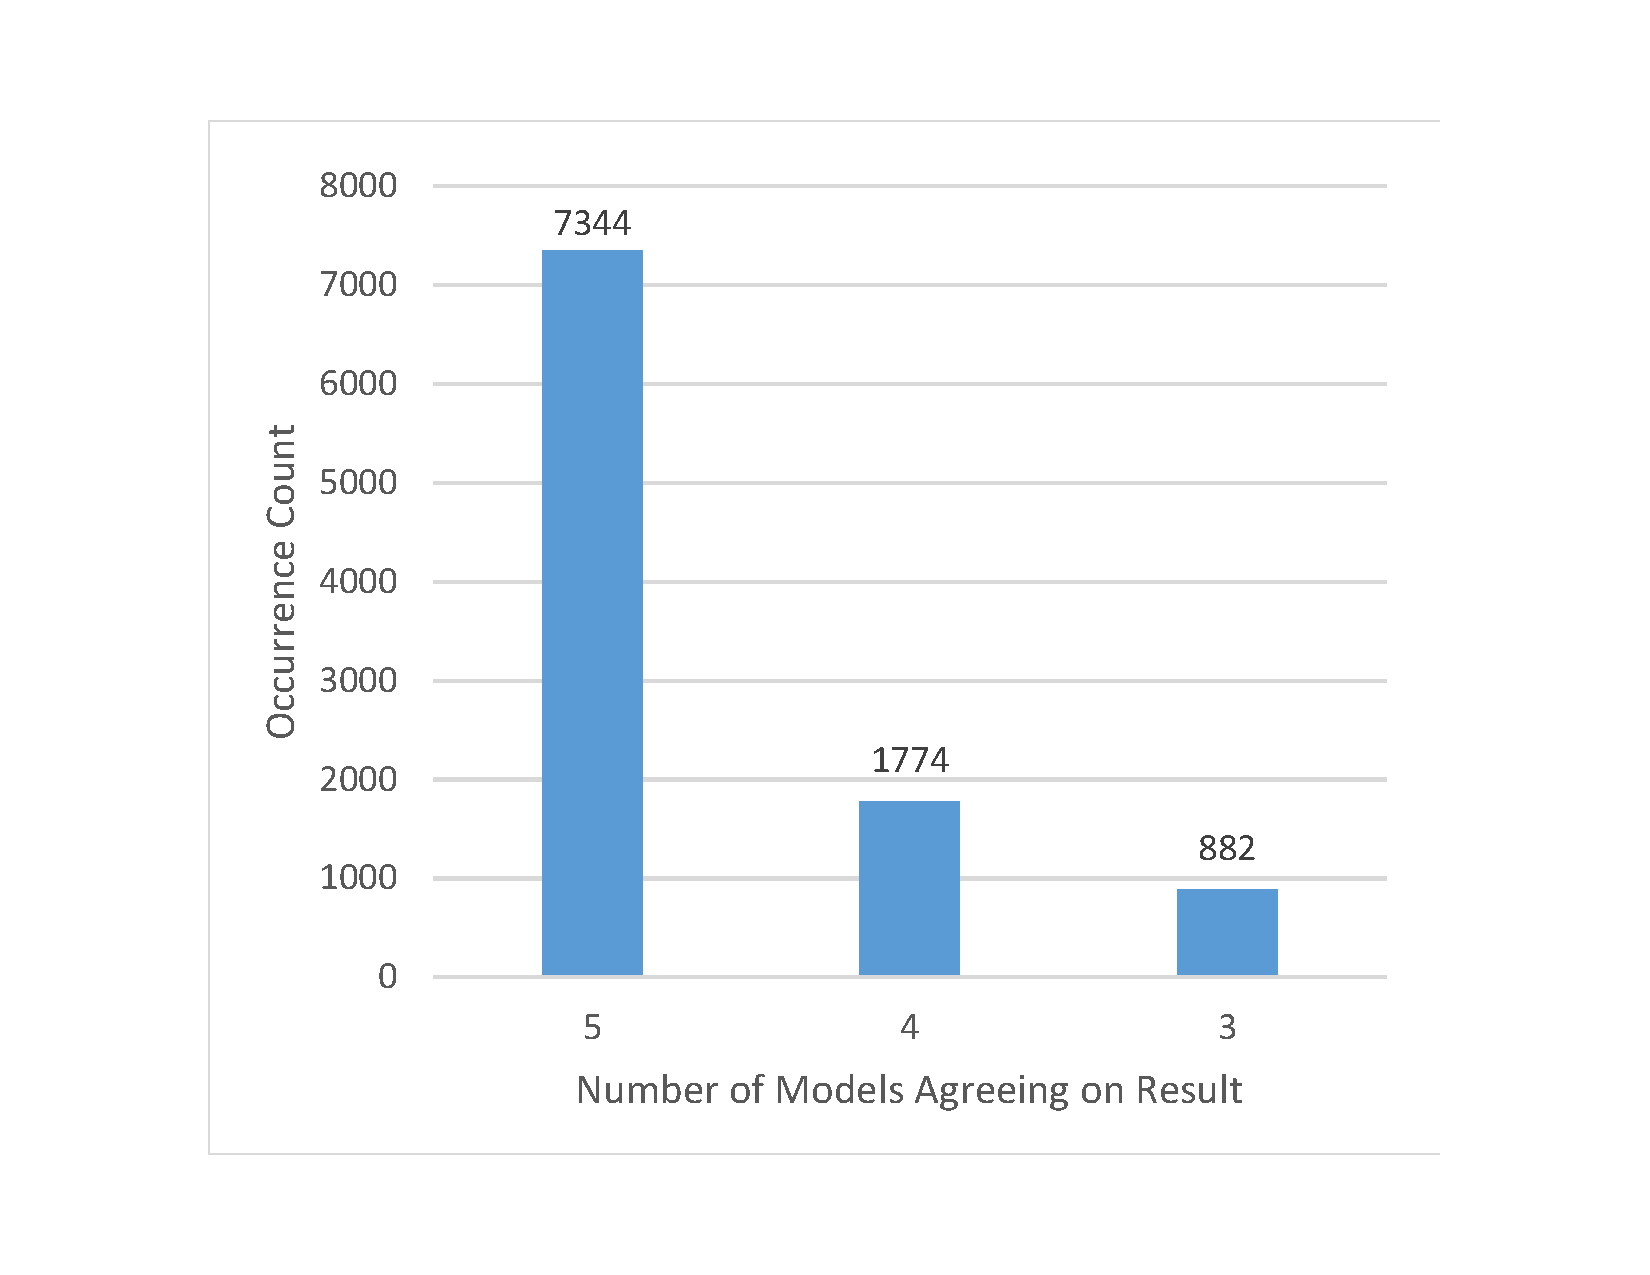
\includegraphics[width=0.5\textwidth]{./ensemble_diag}
\caption{Bar plot of the number of models that ended up voting for the final majority result.}\label{fig:diag}
\end{figure}

Our ensemble model leverages this diversity. The majority voting results are summarized in Figure~\ref{fig:diag}. We can see that in a total of about 26.5\% of the cases, at least one model was unsure about the chosen prediction.

\section{Summary}
To summarize, we have presented several approaches that perform competitively on the task of Twitter sentiment classification.
They consistently outperform the baselines, behave in a stable fashion during training, are simple to implement, and need almost no preprocessing (on top of the already provided and processed data).

We have also shown that the models are diverse, and combining them in an ensemble reduces prediction variance and thus improves generalization.

\section*{Acknowledgements}

We would like to thank the Data Analytics Lab and ETH~Z\"{u}rich for computational resources for this project on the Leonhard cluster, and answering all our questions on Piazza or otherwise.

\bibliographystyle{IEEEtran}
\bibliography{report}

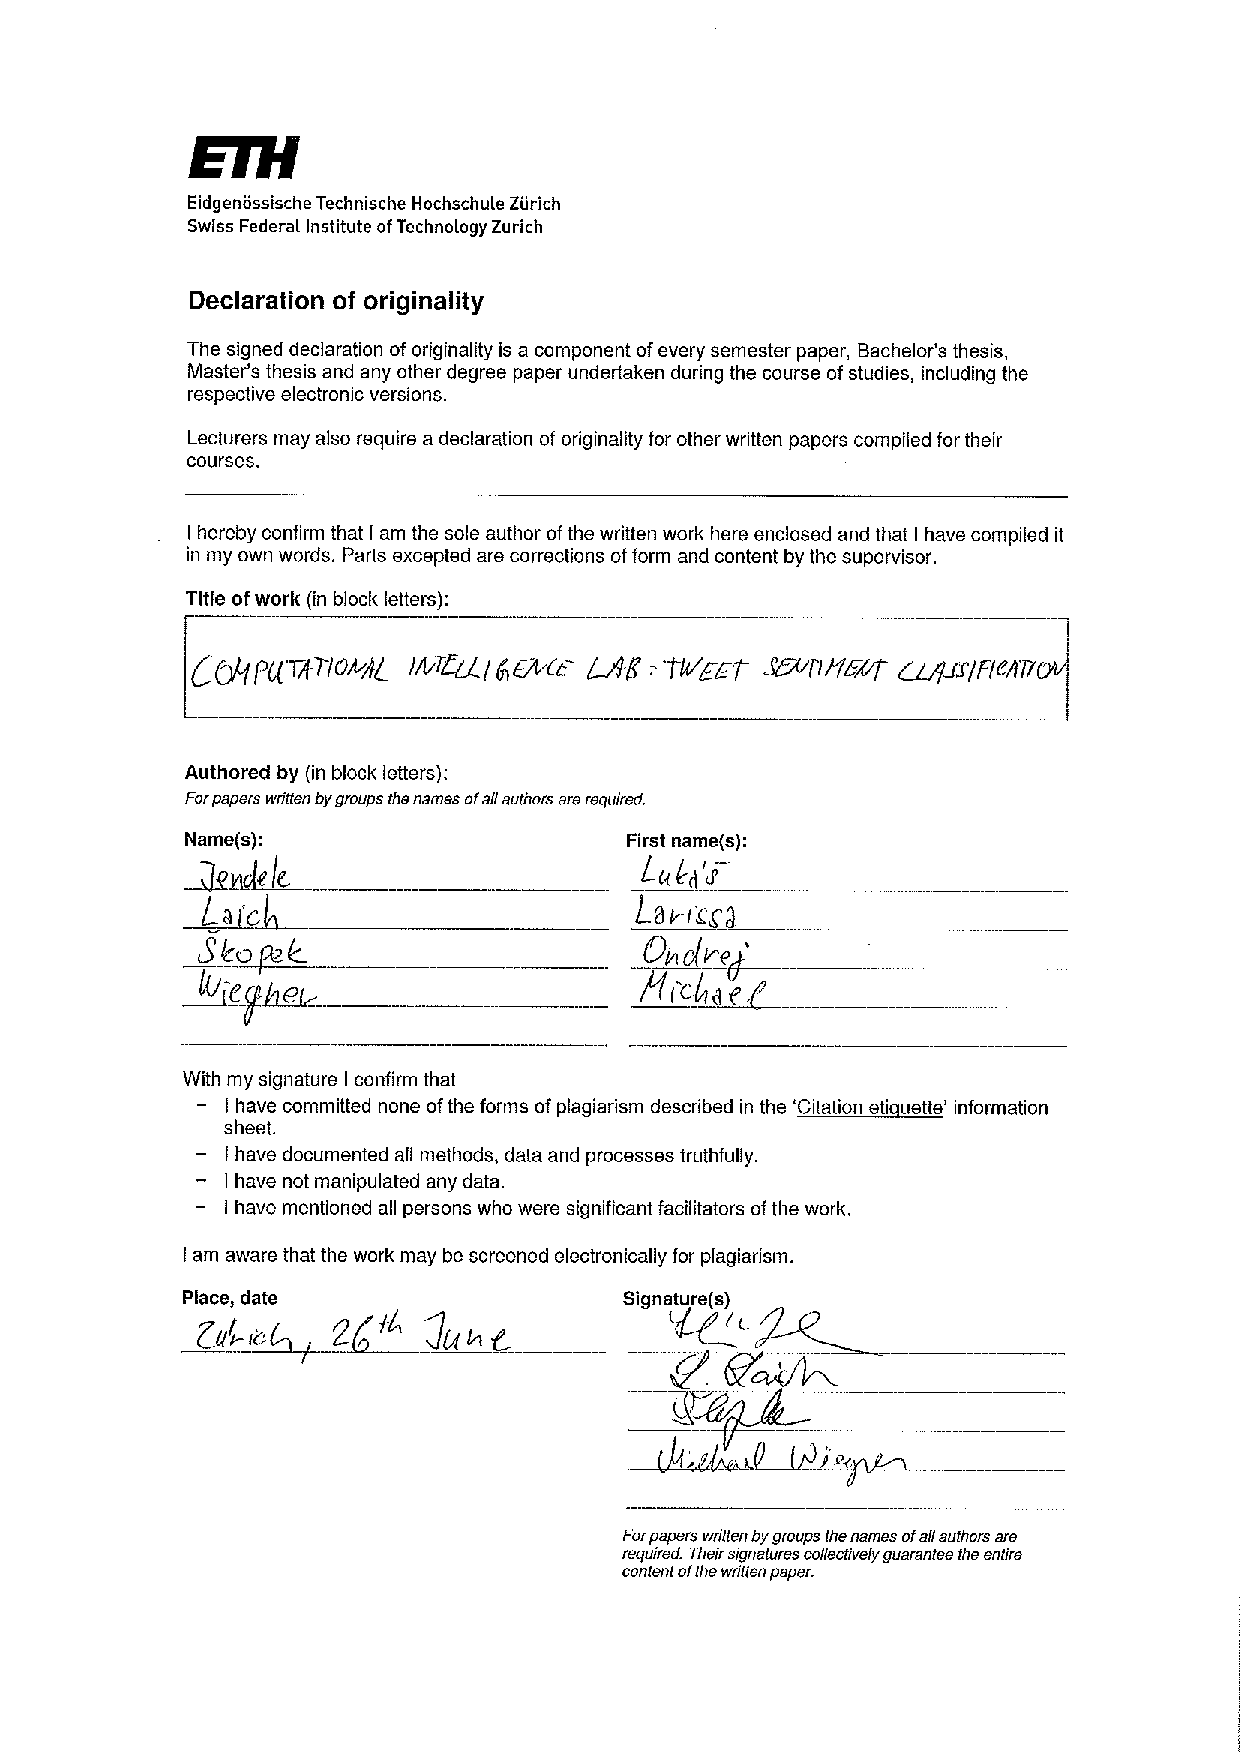
\includepdf[pages=-]{declaration.pdf}
\end{document}

